\begin{sloppypar}\noindent\textbf{Arabic.} The same count for the Arabic Qur'an and hadith with the ArSL lexicon (Table~\ref{tab:coverage_ar})
gives 59.6\% of all word occurrences and 53.3\% of content-word occurrences. Two
differences from English must be kept in mind. First, Arabic attaches conjunctions, prepositions and pronouns to words
(\ar{فقال}, \ar{عنه}, \ar{منها}), so the count of \emph{distinct} surface forms (62,562) is far larger than the number of
lemmas and the distinct-word figure (23.9\%) understates coverage. Second, Arabic has no capital letters, so proper names
cannot be detected the same way and remain in the count: \ar{عمر}, \ar{أبو هريرة}, \ar{عائشة}, \ar{أبو بكر}, \ar{أنس},
\ar{ابن عباس} are among the most frequent uncovered words, together with the formulas \ar{صلى الله عليه وسلم} and
\ar{عز وجل}. The real gaps are content words such as \ar{القيامة}, \ar{الدنيا}, \ar{القرآن} and \ar{شيء}, which are the
next signs to collect. Starting from the 53.3\% of content-word occurrences, the 50, 100, 200 and 500 most frequent uncovered forms would
raise coverage to 64.0\%, 66.5\%, 69.0\% and 72.9\%. (This run counted 3,948 glosses: the 31 letter signs are
excluded.)
\end{sloppypar}

\begin{table}[ht]
\centering\small
\caption{ArSL lexicon coverage of the Arabic Qur'an and hadith corpora. Distinct
counts are of surface forms with clitics.}
\label{tab:coverage_ar}
\begin{tabular}{l l r r r r}
\toprule
Corpus & Words counted & Distinct & Distinct covered & Occurrences & Occurrences covered \\
\midrule
Qur'an & content words & 14,603 & 3,987 (27.3\%) & 62,719 & 29,061 (46.3\%) \\
Qur'an & all words & 14,648 & 4,026 (27.5\%) & 77,800 & 42,445 (54.6\%) \\
Hadith & content words & 55,712 & 13,847 (24.9\%) & 532,303 & 287,855 (54.1\%) \\
Hadith & all words & 55,763 & 13,888 (24.9\%) & 649,535 & 391,346 (60.2\%) \\
Both & content words & 62,562 & 14,979 (23.9\%) & 595,022 & 316,916 (53.3\%) \\
Both & all words & 62,613 & 15,020 (24.0\%) & 727,335 & \textbf{433,791 (59.6\%)} \\
\bottomrule
\end{tabular}
\end{table}

\begin{figure}[ht]
\centering
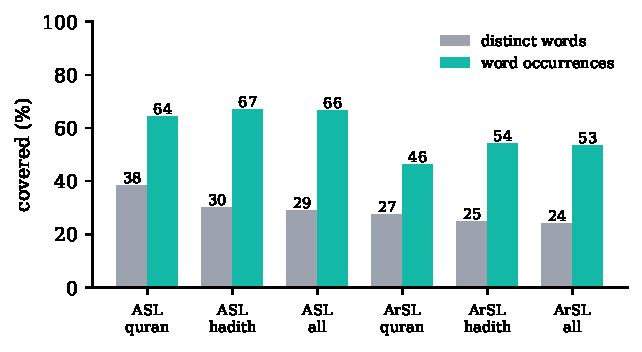
\includegraphics[width=0.7\textwidth]{figures/coverage_bars.pdf}
\caption{Coverage of the Qur'an and hadith by the ASL lexicon (English corpora, vocabulary without names) and the ArSL
lexicon (Arabic corpora, content words). Grey: distinct words; teal: word occurrences.}
\label{fig:covbars}
\end{figure}
